\section{采样理论}\label{sec:采样理论}
数字图像表示为一组像素值,通常对齐到矩形网格。
当在物理设备上展示数字图像时,这些值用于确定显示器上像素发射的光谱功率。
当考虑数字图像时,区分图像像素与显示器像素很重要,
前者表示一个函数在特定样本位置的值,后者是具有某个发光分布的物理对象
(例如对于LCD显示器,当以倾斜角度观察它时,颜色和亮度可能会极大变化)。
显示器用图像像素值在显示器表面构造新的图像函数。
该函数定义在显示器所有点位上,而不只是数字图像像素的无穷小点上。
这样取一组样本值并将其转换回连续函数的过程称为\keyindex{重建}{reconstruction}{}。

为了计算数字图像中的离散像素值,必须采样原始连续定义的图像函数。
在pbrt中,像大多数其他光线追踪渲染器那样,
获取图像函数有关信息的唯一方法就是通过追踪光线来对其采样。
例如,能计算胶片平面上两点间的图像函数变化边界的通用方法是不存在的。
尽管可以通过在像素位置上精确采样该函数来生成图像,
但通过在不同位置上取用更多样本并将这些关于图像函数的
额外信息融合到最终的像素值中能得到更好的结果。
实际上,为了有最佳质量的结果,计算像素值时应使得
在显示设备上重建的图像尽可能与虚拟相机胶片平面上的场景原始图像逼近。
注意这和希望显示器像素在其位置上取用图像函数实际值的目标有些微妙区别。
处理这一区别是本章实现的算法的主要目标
\footnote{本书中我们将忽略物理显示器像素特性相关问题并
在显示器执行本节后面所述理想重建过程的假设下处理。
该假设显然与真实显示器的工作方式不符,但这里它避免了不必要的复杂分析。
\citet{GLASSNER1995}的第3章很好地处理了非理想显示设备
及其对图像采样和重建过程的影响。}。

因为采样和重建过程涉及估值,所以它引入了称作\keyindex{混叠}{aliasing}{}的误差,
并会以许多方式表现出来,包括锯齿状边缘或动画中的闪烁。
产生这些误差的原因是采样过程不能捕获来自连续定义的图像函数的全部信息。

作为这些思想的一个例子,考虑一个1D函数(我们也会称之为信号)即$f(x)$,
我们可以求函数定义域中任意期望位置$x'$处的值$f(x')$。
每个这样的$x'$称为\keyindex{样本位置}{sample position}{},
$f(x')$的值称为\keyindex{样本值}{sample value}{}。
\reffig{7.1}展示了光滑1D函数的样本集,以及逼近原始函数$f$的重建信号$\tilde{f}$。
本例中,$\tilde{f}$是分段线性函数,通过线性插值相邻样本值来逼近$f$
(已经熟悉采样理论的读者会认出这是用帽函数\sidenote{译者注:原文hat function。}重建的)。
因为关于$f$唯一可用的信息是来自在位置$x'$处的采样值,
且没有关于$f$在样本间特性的信息,所以$\tilde{f}$不可能完全匹配$f$。
\begin{figure}[htbp]
    \centering
    \subfloat[]{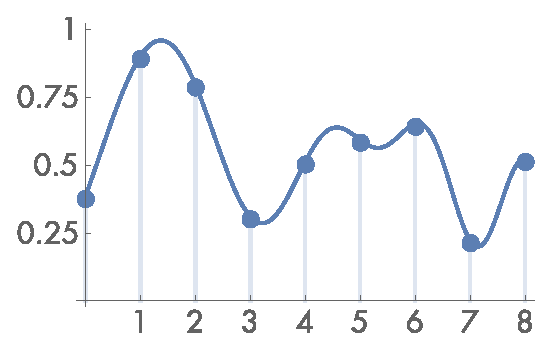
\includegraphics[width=0.45\linewidth]{chap07/point-sampling.eps}}\,
    \subfloat[]{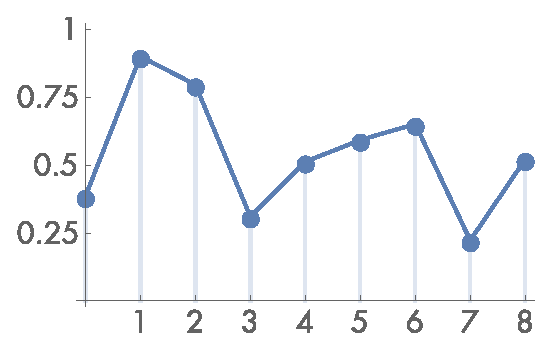
\includegraphics[width=0.45\linewidth]{chap07/linear-reconstruction.eps}}
    \caption{(a)通过取$f(x)$的\emph{样本点}集(标实心记),我们确定了函数在这些位置处的值。
    (b)样本值可用于\emph{重建}逼近$f(x)$的函数$\tilde{f}(x)$。
    \refsub{混叠}介绍的采样原理准确描述了关于$f(x)$的条件、
    所需样本的数目,以及使得$\tilde{f}(x)$和$f(x)$一模一样的重建技术。
    原始函数有时能只从样本点中完全重建的事实令人瞩目。}
    \label{fig:7.1}
\end{figure}

\keyindex{傅里叶分析}{Fourier analysis}{}可用于评估重建函数与原始函数间的匹配质量。
本节将用丰富细节来介绍一部分采样和重建过程中涉及的傅里叶分析主要思想,
但略去了许多性质的证明并跳过了与pbrt所用的采样算法没有直接关系的细节。
本章“扩展阅读”一节有关于这些话题详细信息的指引。

\subsection{频域与傅里叶变换}\label{sub:频域与傅里叶变换}

\subsection{混叠}\label{sub:混叠}